% --- tv2_quangvinh.tex ---
% Phân tích Nhóm 2: Phân tích Sản phẩm & Danh mục

\noindent\textbf{3. Kết quả phân tích \& Trực quan hóa:}

\begin{figure}[H]
    \centering
    
\includegraphics[width=0.8\textwidth]{images/category_finance/cat_revenue.png}
    \caption{Tổng doanh thu theo từng danh mục sản phẩm}
    \label{fig:cat_revenue}
\end{figure}

\textbf{a. Phân tích Doanh thu theo Danh mục}
\\
Biểu đồ \ref{fig:cat_revenue} cho thấy sự phân hóa cực kỳ rõ rệt về doanh thu giữa các nhóm ngành hàng. Danh mục \textbf{Electronics (Điện tử)} áp đảo hoàn toàn với tổng doanh thu đạt mức \$3.31 triệu, cao gấp 3 lần so với nhóm xếp thứ hai là \textbf{Home (Nhà cửa)} (\$1.07 triệu). Các nhóm hàng tiêu dùng thiết yếu như Grocery (Tạp hóa) lại có doanh thu thấp nhất (\$82 nghìn). Điều này chỉ ra rằng các sản phẩm điện tử, dù có số lượng giao dịch thể không quá cao, nhưng nhờ đơn giá lớn đã mang lại nguồn thu khổng lồ cho nền tảng.

\begin{figure}[H]
    \centering
    
\includegraphics[width=0.8\textwidth]{images/category_finance/cat_return_rate.png}
    \caption{Tỷ lệ hoàn trả (Return Rate) theo danh mục}
    \label{fig:cat_return}
\end{figure}

\textbf{b. Phân tích Rủi ro Hoàn trả (Return Rate)}
\\
Biểu đồ \ref{fig:cat_return} thể hiện phần trăm các đơn hàng bị trả lại trên tổng số đơn. Có một điều đáng lưu ý là \textbf{Fashion (Thời trang)} dẫn đầu bảng với tỷ lệ hoàn trả cao nhất lên tới 8.28\%, theo ngay sau là \textbf{Electronics} (7.29\%). Đối với ngành thời trang, tỷ lệ trả hàng cao thường xuất phát từ vấn đề sai lệch kích cỡ hoặc không ưng ý về kiểu dáng. Đối với đồ điện tử, đây có thể là rủi ro liên quan đến lỗi kỹ thuật. Trong khi đó, nhóm \textbf{Grocery} có tỷ lệ trả hàng thấp nhất (chỉ 1.3\%), cho thấy vòng đời sử dụng nhanh và ít sai số.

\begin{figure}[H]
    \centering
    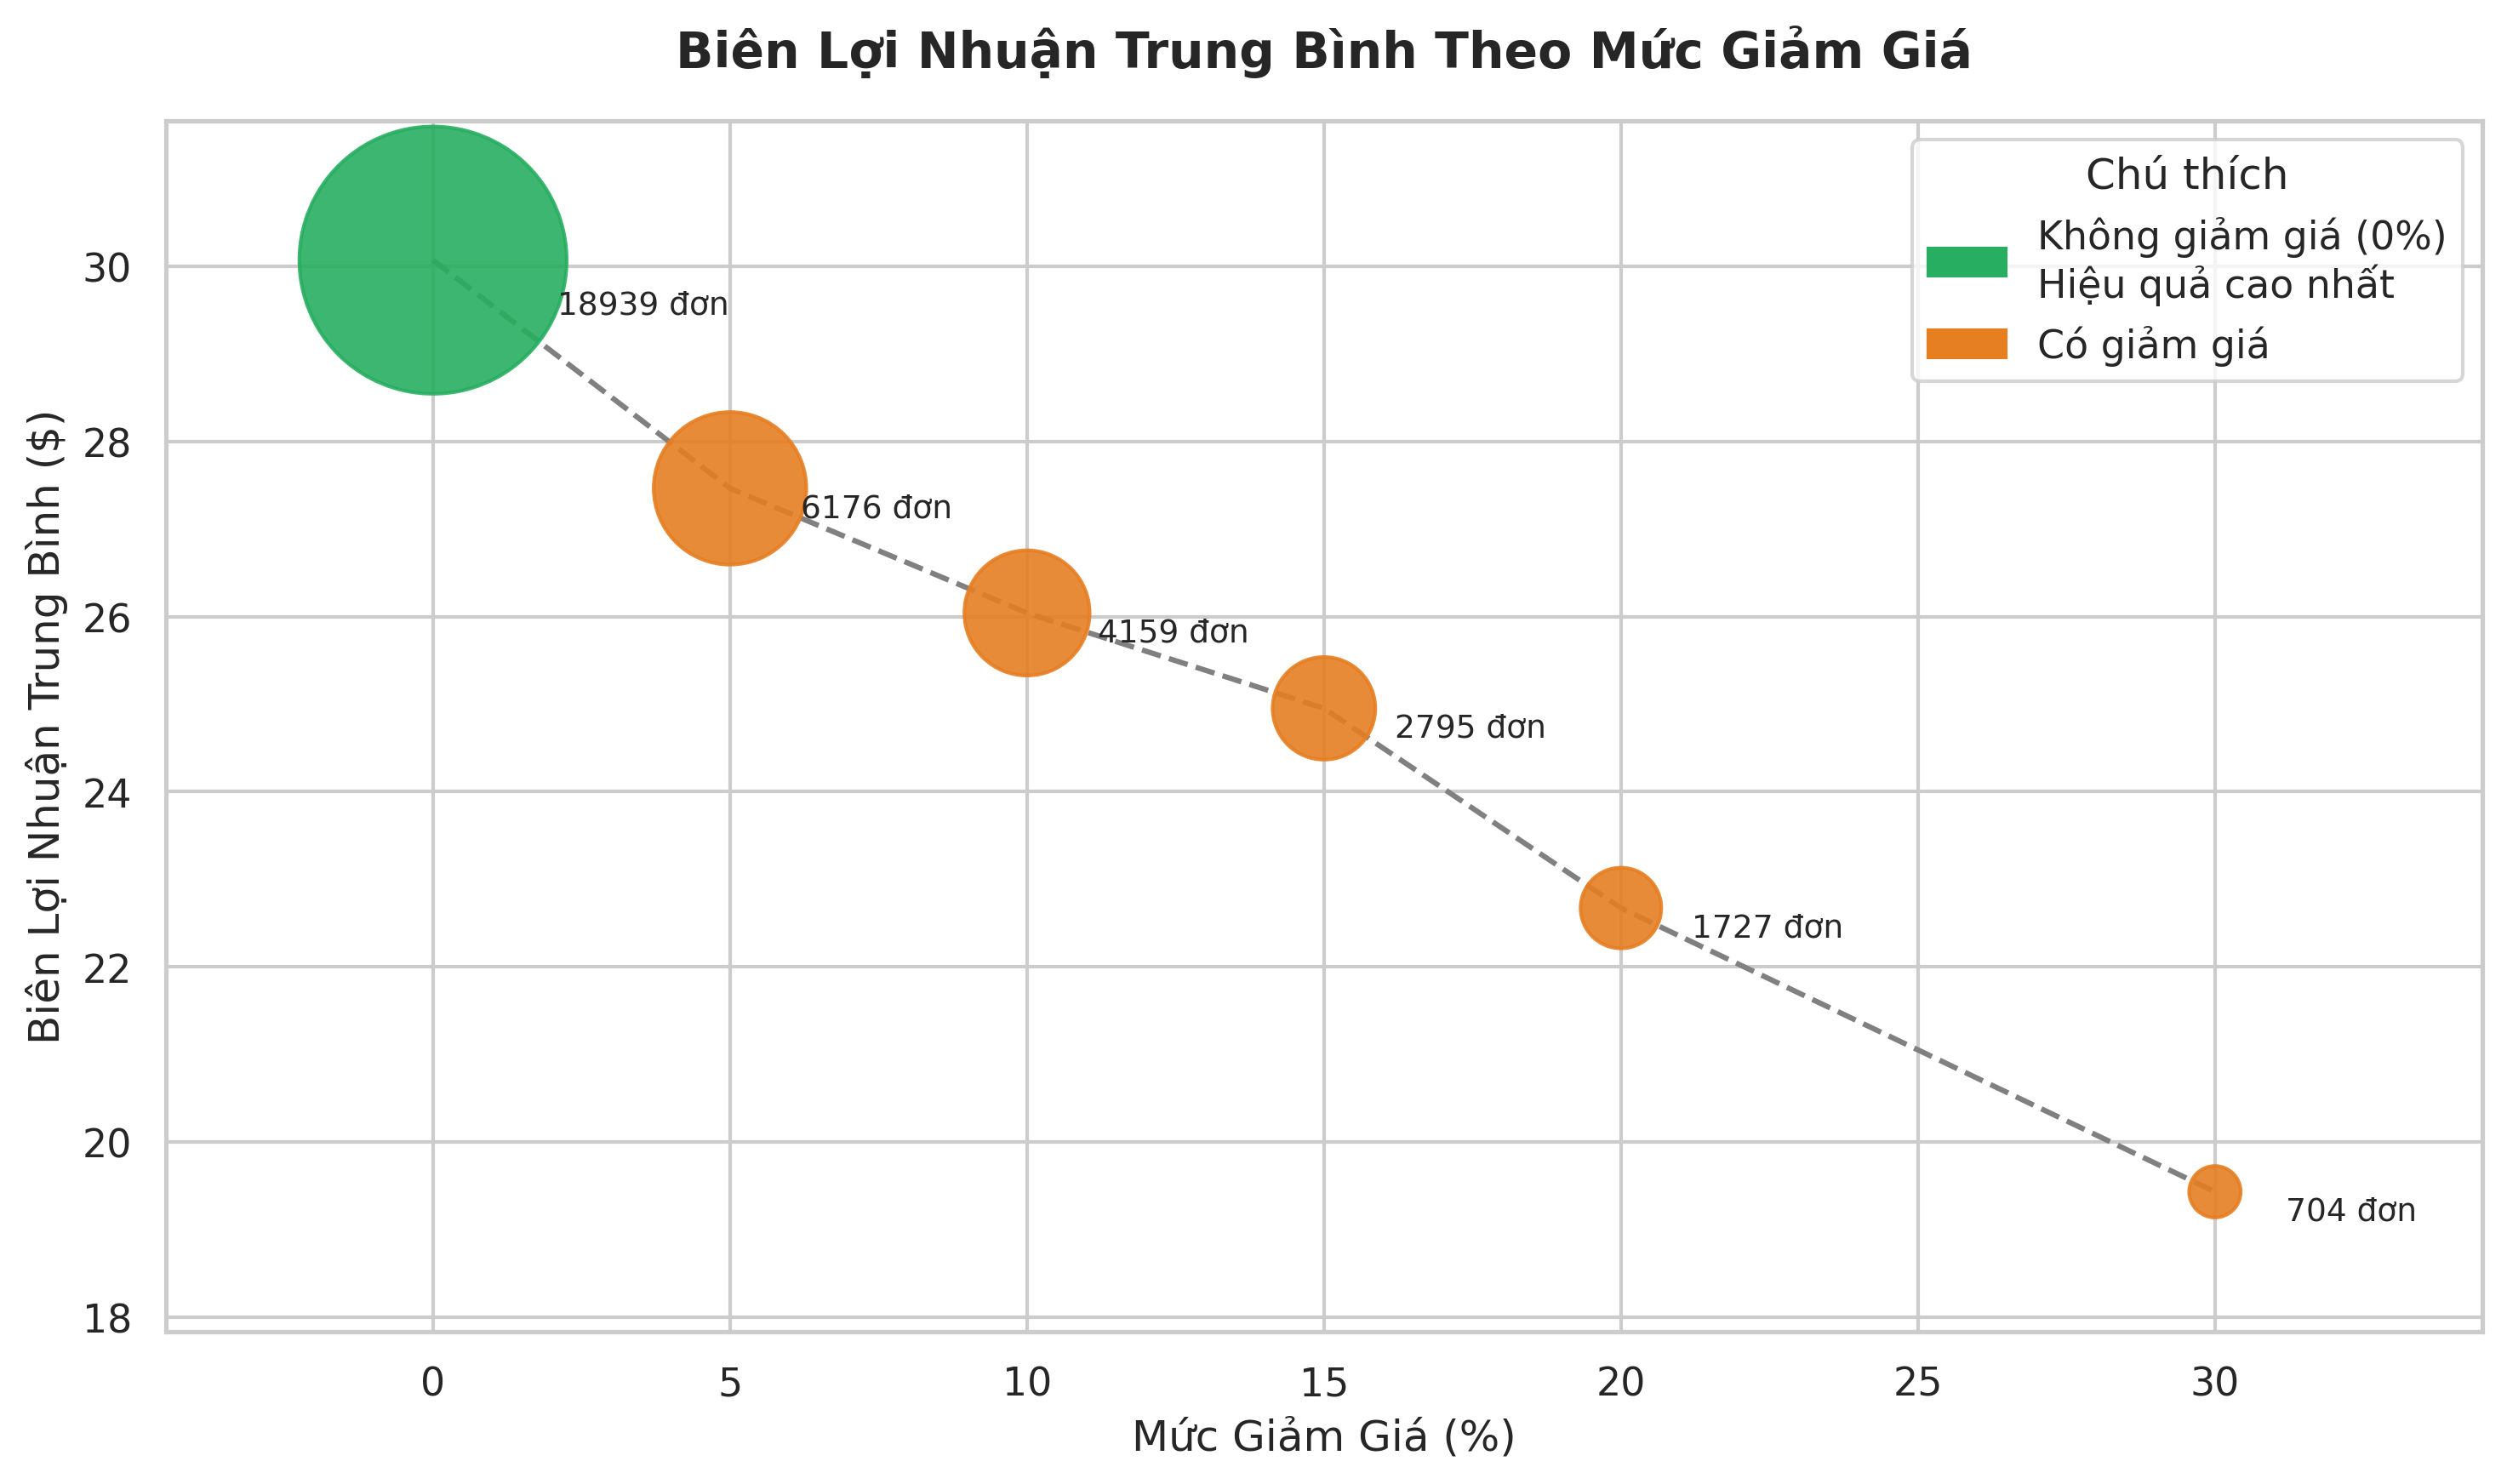
\includegraphics[width=0.8\textwidth]{images/category_finance/discount_profit.png}
    \caption{Mối tương quan giữa phần trăm giảm giá và biên lợi nhuận trung bình}
    \label{fig:discount_profit}
\end{figure}

\textbf{c. Tương quan giữa Mức Giảm Giá và Biên Lợi Nhuận}
\\
Thông qua biểu đồ phân tán \ref{fig:discount_profit} (kích thước điểm ảnh biểu diễn số lượng đơn hàng), ta dễ dàng nhận thấy một quy luật tuyến tính nghịch biến: \textbf{Mức giảm giá càng cao, biên lợi nhuận trung bình cho mỗi đơn hàng càng giảm}.
Đáng chú ý, đa số các đơn hàng (gần 19,000 đơn) không áp dụng mã giảm giá (0\%) và đem lại biên lợi nhuận cao nhất (khoảng \$30.07). Trong khi đó, các mức giảm giá sâu như 30\% khiến biên lợi nhuận sụt giảm xuống chỉ còn \$19.42 và số lượng giao dịch tại mức này cũng rất ít (hơn 700 đơn). Do đó, doanh nghiệp cần cân nhắc kỹ việc lạm dụng khuyến mãi sâu vì nó gây tổn thất đáng kể đến lợi nhuận ròng mà không tạo ra đột biến ấn tượng về số lượng đơn hàng.

\vspace{0.3cm}
\noindent\textbf{4. Đưa ra quyết định trong tương lai:}
\begin{itemize}
    \item \textbf{Tối ưu danh mục chủ lực:} Tập trung nguồn lực marketing và đa dạng hóa mẫu mã cho nhóm \textbf{Electronics} vì đây là "mỏ neo" doanh thu chính. Tuy nhiên, cần thắt chặt kiểm tra kỹ thuật trước khi giao để giảm tỷ lệ hoàn trả (7.29\%).
    \item \textbf{Cải thiện chất lượng ngành Fashion:} Triển khai thêm các công cụ hỗ trợ chọn size hoặc mô tả chi tiết hơn để giảm thiểu tỷ lệ hoàn trả cao nhất hệ thống (8.28\%).
    \item \textbf{Chiến lược chiết khấu:} Ưu tiên các mức giảm giá từ 0--10\% để duy trì biên lợi nhuận ổn định. Tránh các chương trình giảm giá sâu (trên 20\%) trừ khi mục tiêu là xả kho vì hiệu quả mang lại về lợi nhuận là không cao.
\end{itemize}

